\chapter{Definita integraler}
Den efinita integralen $\int_a^b f(x)\, dx$ av en kontinuerlig funktion
$f$ över ett intervall $[a,b]$ definieras som det \underline{unika tal}
$I$ som alltid ligger mellan godtycklig nedåt begränsad- och övrebegränsad Riemannsumma (om det finns):
\begin{equation*}
    L(f,P)\leq I \leq U(f,P)
\end{equation*}
för \underline{alla} tänkbara partitioner $P$ av $[a,b]$.\\
Geometriskt tolkas $\int_a^b f(x)\, dx$ som "arean under grafen till $f$ med tecken".\\
%infoga bild 1
% 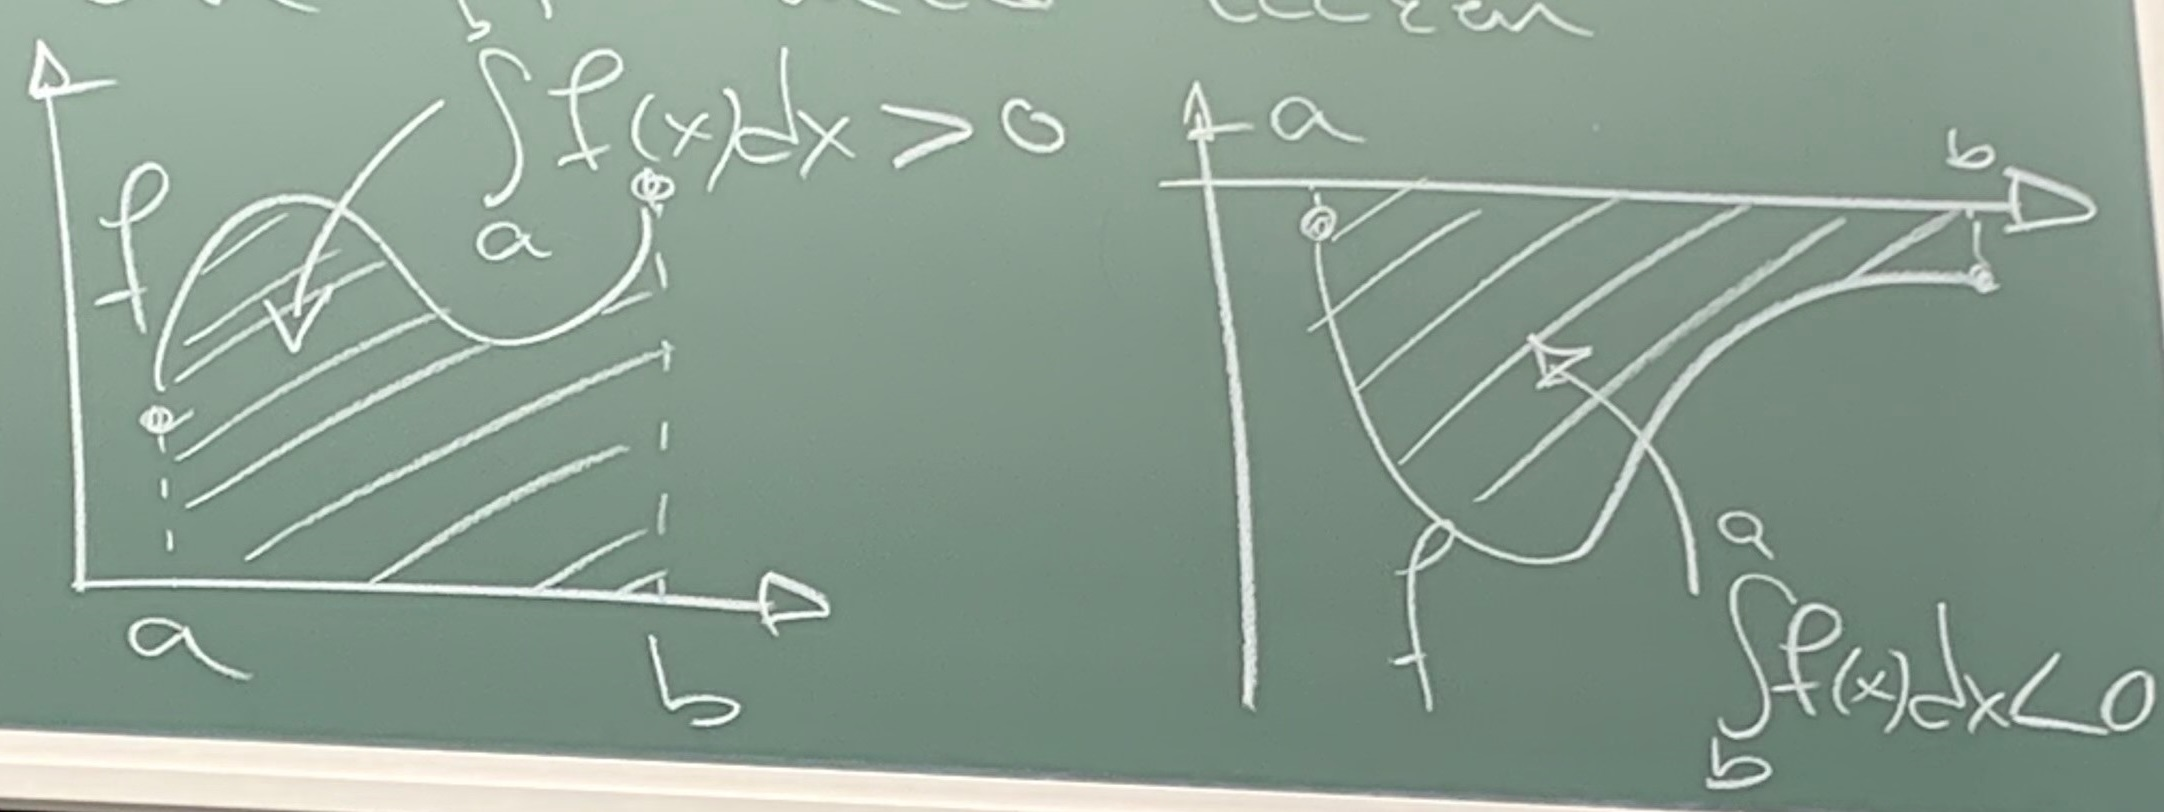
\includegraphics{lessons/lesson15/imgs/img01.jpg}\\

Har här förutsatt att $a<b$, men är naturligt att utvidga konceptet med definit intergral genom följande definitioner:
\begin{itemize}
    \item $a=b\Rightarrow \int_a^b f(x)\, dx = 0$
    \item $a>b\Rightarrow \int_a^b f(x)\, dx = - \int_a^b f(x)\, dx$
\end{itemize}
Integrering är en \underline{linjär} operation, dvs. superpositionsprincipen gäller:
\begin{equation*}
    \int_{a}^{b} \alpha \cdot f(x) +\beta \cdot g(x) \, dx =
    \alpha \int_{a}^{b} f(x)\, dx + \beta \int_{a}^{b} g(x)\, dx
\end{equation*}
för alla $\alpha,\beta\in\mathbb{R}$.
Rent geometriskt gäller också följande:
\begin{itemize}
    % infoga bild 2
    \item $\Rightarrow \int_a^c f(x)\, dx = \int_a^b f(x)\, dx + \int_b^c f(x)\, dx$
          % infoga bild 3
    \item $\Rightarrow \int_a^b f(x)\, dx \leq \int_a^b g(x)\, dx$
          % infoga bild 4
    \item $\Rightarrow |\int_a^b f(x)\, dx| \leq \int_a^b |f(x)|\, dx$ (triangelolikheten)
          %infoga bild 5
    \item $\Rightarrow \int_{a-b}^{a+b} f(x)\, dx = 2\cdot\int_{a-b}^{a} f(x)\, dx = 2\cdot\int_{a}^{a+b} f(x)\, dx$\\
          $f$ \underline{jämn} med avseende på $x=a$
          %infoga bild 6
    \item $\Rightarrow \int_{a-b}^{a+b} f(x)\, dx = 0$\\
          $f$ \underline{udda} med avseende på $x=a$
\end{itemize}

För kontinuerliga funktioner och för derivator gäller "medelvärdessatser".
\begin{itemize}
    \item $f$ kontinuerlig på $[a,b] \Rightarrow$ det finns en punkt $c\in[a,b]$ där $f$ antar värdet $\frac{f(a)-f(b)}{2}$
    \item $f$ deriverbar på $(a,b)\Rightarrow$ det finns en punkt $c\in(a,b)$ där derivatan av $f$ motsvarar snittlutningen på intervallet,
          dvs. $f^\prime(c)=\frac{f(b)-f(a)}{b-a}$
\end{itemize}

Analog medelvärdessats finns också för definita integraler!

\paragraph*{Sats (Medelvärdessatsen för definita integraler)}
Om $f$ är kontinuerlig på $[a,b]$ så finns en punkt $c\in[a,b]$ så att
\begin{equation*}
    \int_a^b f(x)\, dx = (b-a) \cdot f(c)
\end{equation*}
Medelvärdessatsen för integraler säger att det finns en rektangel med bred $b-a$ och höjd $f(c)$ (för något $c\in[a,b]$) vars area är precis $\int_a^b f(x)\, dx$.\\
%infoga bild 7
% 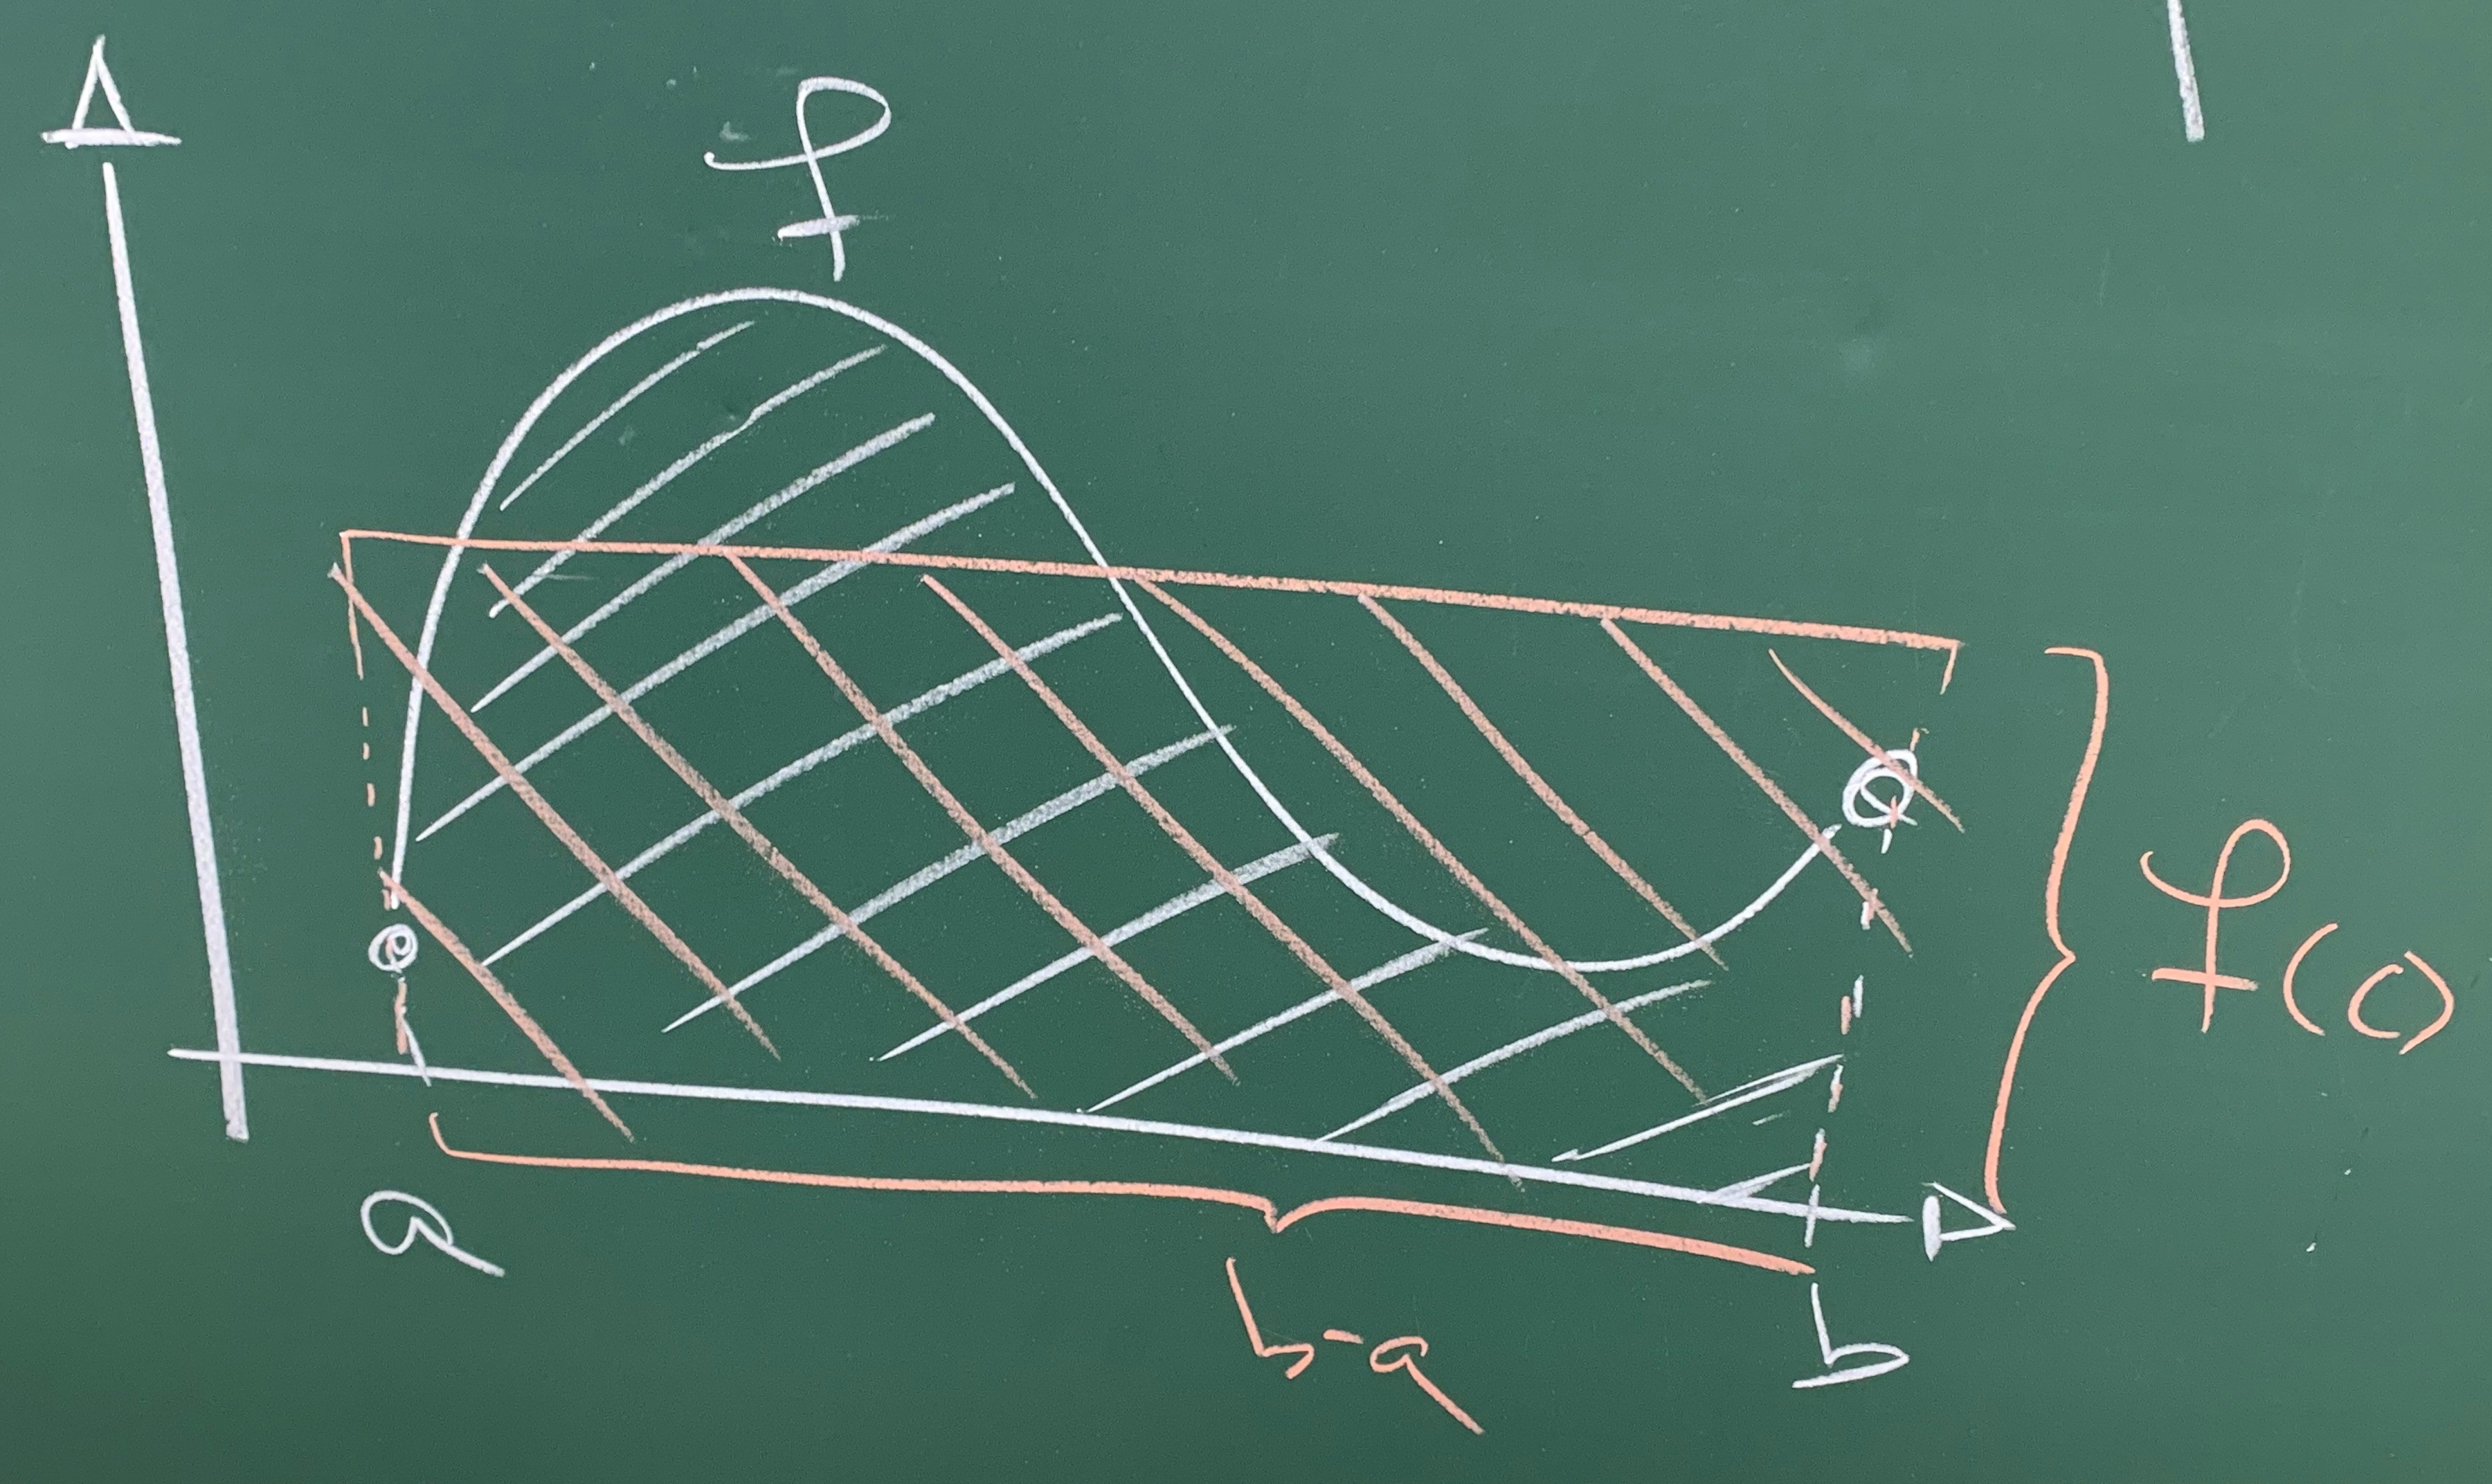
\includegraphics[]{lessons/lesson15/imgs/img07.jpg}\\
Ur detta resultat \underline{definieras} medelvärdet av en funktion $f$ (integrerbar) på ett intervall $[a,b]$ som:
$\overline{f}\frac{1}{b-a}\cdot \int_a^b f(x)\, dx$ (rimligare än t.ex. att sätta medelvärdet som $\frac{f(a)+f(b)}{2}$ eftersom integralen tar hänsyn till $f$ över \underline{hela} intervallet $[a,b]$ och inte bara ändpunkterna).

\chapter{Analysens huvudsats}
Att definiera integraler genom Riemann-summor är bra på många sätt, inte minst för att det är intuitivt, men vi måste ha ett smidigare sätt att beräkna $\int_a^b f(x)\, dx$ (håller ej att behöva beräkna gränsvärdet $L(f,P)$ och $U(f,P)$).
Detta löser delvis analysens huvudsats.

\paragraph*{Sats (Analysen huvudsats) (tenta)}
Antaga att funktionen $f$ är kontinuerlig på ett intervall $I$ som innehåller punkten $a$.
\begin{enumerate}
    \item Låt $F$ vara en funktion på $I$ definierat som $F(x)=\int_a^xf(t)\, dt$
          Då är $F$ deriverbar på $I$ och $F^\prime(x)=f(x)$, dvs.
          \begin{equation*}
              \frac{d}{dx}\int_a^x f(t)\,dt=f(x)
          \end{equation*}
          (så derivering är "antioperationen" till integrering!)
    \item Om $G(x)$ är en primitiv funktion till $f(x)$ på $I$,
          dvs. $G^\prime(x)=f(x)$ så gäller för varje $b\in I$ att:
          \begin{equation*}
              \int_a^b f(x)\,dx=G(b)-G(a)
          \end{equation*}
          (dvs. en beräkningsformel för integraler)
\end{enumerate}
\subparagraph{Bevis}

\begin{enumerate}
    \item Med definitionen av funktionen $F$ enligt satsen gäller att:
          \begin{equation*}
              F^\prime(x)=\lim_{h\to 0}\frac{F(x+h)-F(x)}{h}=
              \lim_{h\to 0}\frac{1}{h}(\int_a^{x+h}f(t)\, dt - \int_a^x f(t)\, dt)=
          \end{equation*}
          \begin{equation*}
              lim_{h\to 0}\frac{1}{h}\in_x^{x+h} f(t)\, dt=
              \{\text{medelvärdessatsen för integraler}\}=
          \end{equation*}
          \begin{equation*}
              \lim_{h\to 0}\frac{1}{h}(x+h-x)\cdot f(c)=
              \lim_{h\to 0}\frac{1}{h}\cdot h\cdot f(c)=\lim_{h\to 0}f(c)
          \end{equation*}
          för något tal $c\in[x,x+h]$.
          Men vi vet att $f$ är kontinuerlig på intervallet $I$ och
          därmed att $\lim_{h\to 0}f(c)=f(x)$ och alltså är
          $F^\prime(x)=f(x)$ dvs. att $\frac{d}{dx}\int_a^xf(t)\, dt= f(x)$ $\Box$
    \item Om $G^\prime = f(x)$ så är $F(x)=G(x)+C$ på $I$ för något tal
          $C\in\mathbb{R}$ (eftersom två olika primitiva funktioner till
          $f$ endast kan skilja på konstanten).
          Alltså gäller att $\int_a^x f(t)\, dt=G(x)+C$ och om $x=a\Rightarrow 0=G(a)-C$ så $C=-G(a)$-
          Om vi nu sätter $x=b$ får vi att $\int_a^b f(x)\, dx=G(b)-G(a)$ $\Box$
\end{enumerate}

\paragraph{Ex (5.5.15)} Beräkna $\int_0^e a^x\, dx$ $a>0$
\subparagraph{Lösning}
För att lösa problemet vill vi hitta en primitiv funktion till $a^x$,
dvs. $\int a^x\, dx$.
Det gäller att $a^x=e^{ln(a^x)}=e^{x\cdot ln(a)}$. Men $\frac{d}{dx}(e^{x\cdot ln(a)})=ln(a)\cdot e^{x\cdot ln(a)}$
så $\int e^{x\cdot ln(a)}\, dx= \frac{1}{ln(a)}\cdot x^{x\cdot ln(a)}=\frac{a^x}{ln(a)}$.
Så enligt analysens huvudsats gäller $\int_0^e a^x\, dx=[\frac{a^x}{ln(a)}]_0^e=\frac{e^e}{ln(a)}-\frac{a^0}{ln(a)}=\frac{1}{ln(a)}\cdot (a^e-1) \Box$